\usetikzlibrary{calc}
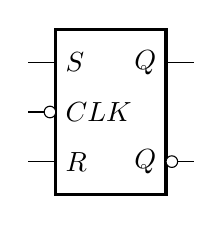
\begin{tikzpicture}[scale=0.7]
  \draw[line width=1.2] (0, 0) rectangle (2, 3);

  \draw ($(0, 0)!0.8!(0,3)$) coordinate (s) -- ++(left:0.5);
  \draw ($(0, 0)!0.5!(0,3)$) coordinate (clk) -- ++(left:0.5);
  \draw ($(0, 0)!0.2!(0,3)$) coordinate (r) -- ++(left:0.5);
  \draw ($(2, 0)!0.8!(2,3)$) coordinate (q) -- ++(right:0.5);
  \draw ($(2, 0)!0.2!(2,3)$) coordinate (nq) -- ++(right:0.5);

  \node[right] at (s) {$S$};
  \node[right] at (r) {$R$};
  \node[right] at (clk) {$CLK$};
  \node[left] at (q) {$Q$};
  \node[left] at (nq) {$Q$};

  \draw[fill=white,draw=black] ($(nq)+(3pt,0)$) circle (3pt);
  \draw[fill=white,draw=black] ($(clk)-(3pt,0)$) circle (3pt);
\end{tikzpicture}
